% compile this file with xelatex
\documentclass[12pt]{article}
\usepackage{graphicx}
\usepackage[margin=2cm, a4paper]{geometry}
\usepackage{setspace}
\usepackage{pdfpages}
\usepackage{float}
\usepackage{xeCJK}
\setCJKmainfont{Noto Serif TC}
\usepackage{amsmath}
\usepackage{fancyvrb}
\usepackage{amssymb}
\usepackage{minted}
\usepackage[colorlinks,linkcolor=blue]{hyperref}
\renewcommand{\contentsname}{Contents}
\renewcommand{\figurename}{Figure}
\renewcommand{\tablename}{Table}
\hypersetup{
    colorlinks=true,
    linkcolor=black,
    filecolor=magenta,      
    urlcolor=blue,
}
\newcommand{\mytitle}{網路管理與系統管理 Lab 13}
\newcommand{\myauthor}{B13902022 賴昱錡}

\usepackage{fancyhdr}
\pagestyle{fancy}
\fancyhead{}
\fancyhead[L]{\mytitle}
\fancyhead[R]{\myauthor}

\title{\mytitle}
\author{\textbf{\myauthor}}
\date{\today}

\begin{document}

\onehalfspacing
\maketitle

\section{The scoreboard}
\begin{figure}[H]
    \centering
    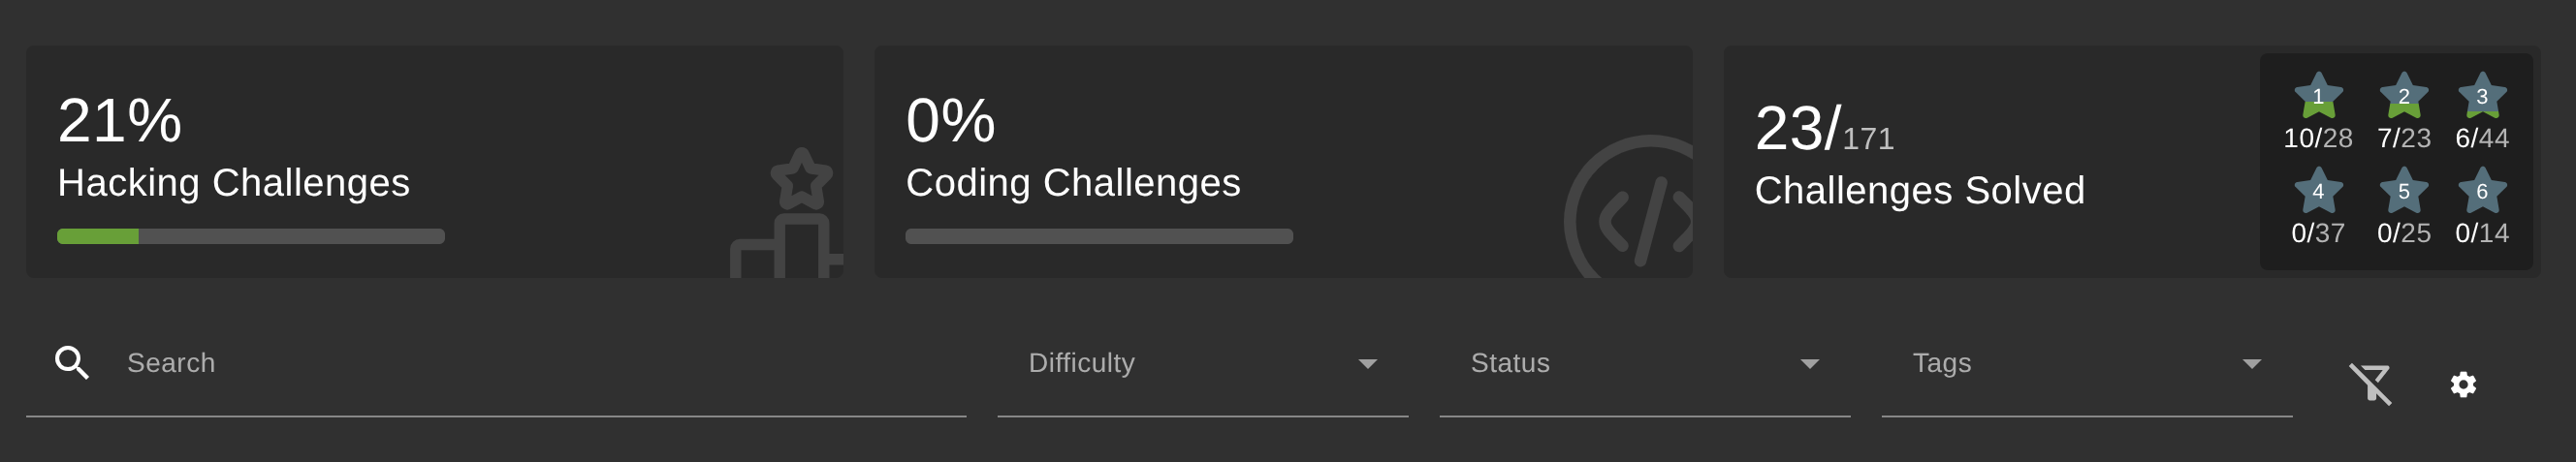
\includegraphics[width=1.0\linewidth]{images/image.png}
    \caption{count of solved problems}
\end{figure}
\begin{figure}[H]
    \centering
    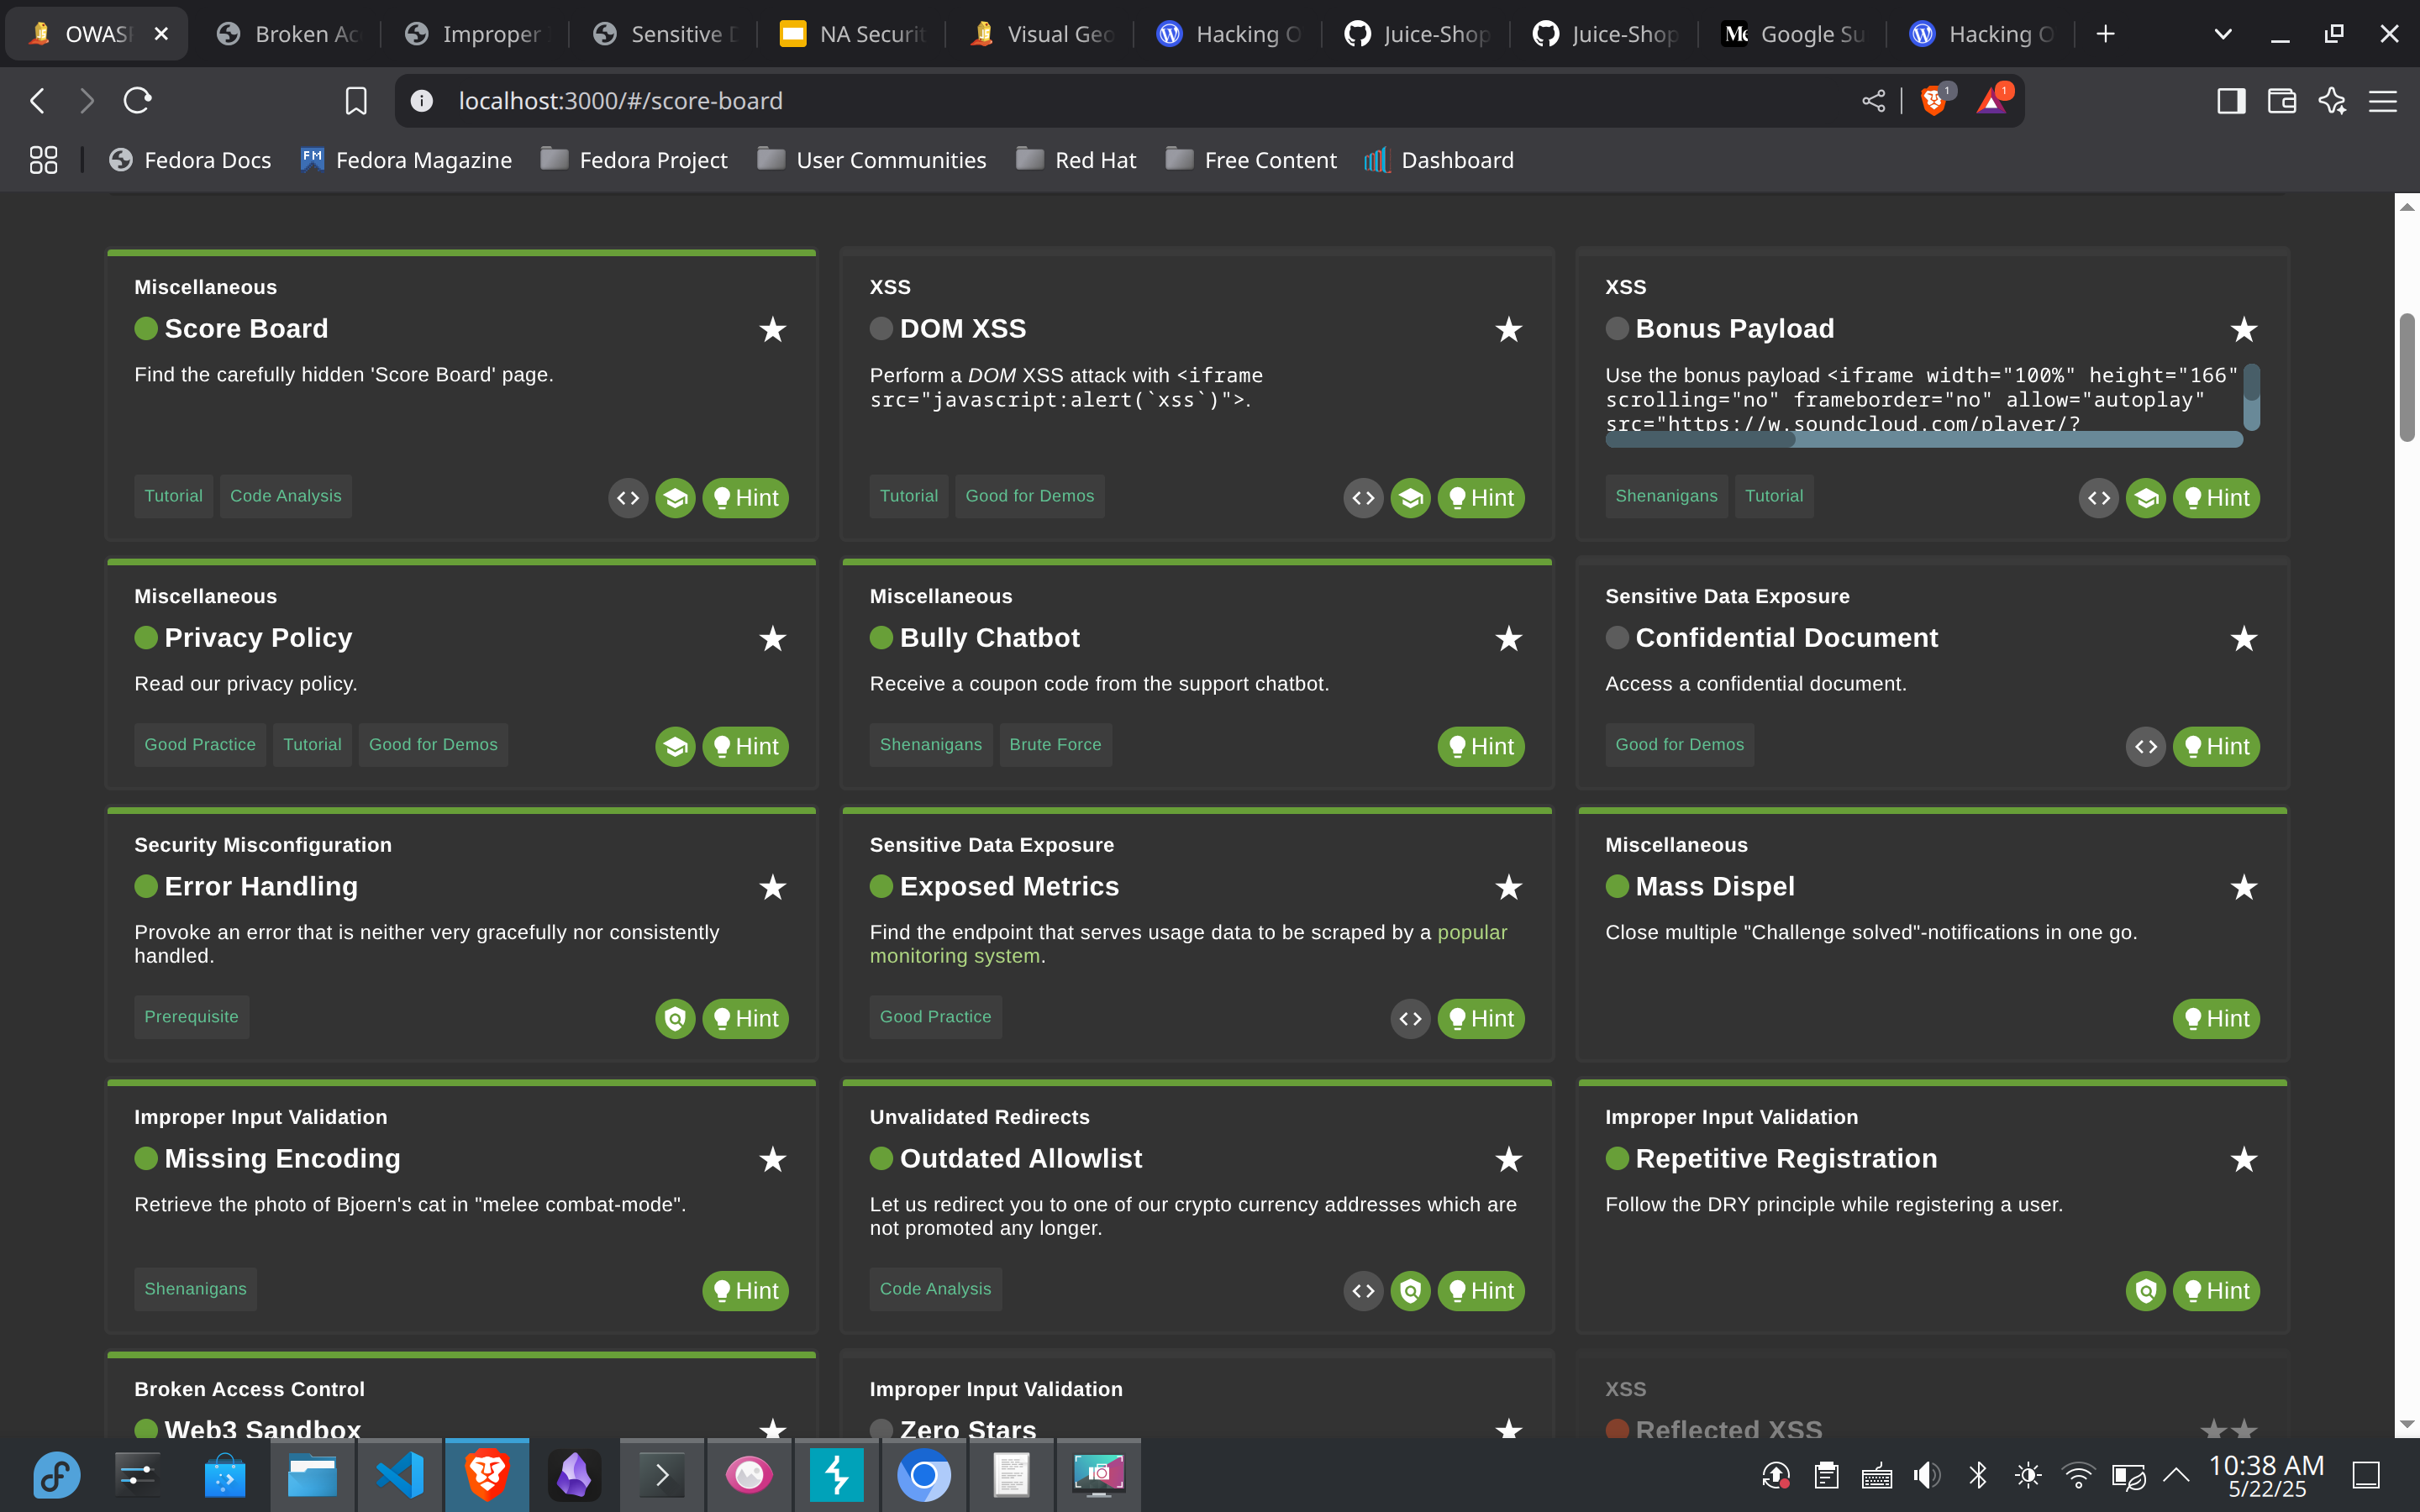
\includegraphics[width=1.0\linewidth]{images/image copy.png}
    % \caption{Caption}
\end{figure}
\begin{figure}[H]
    \centering
    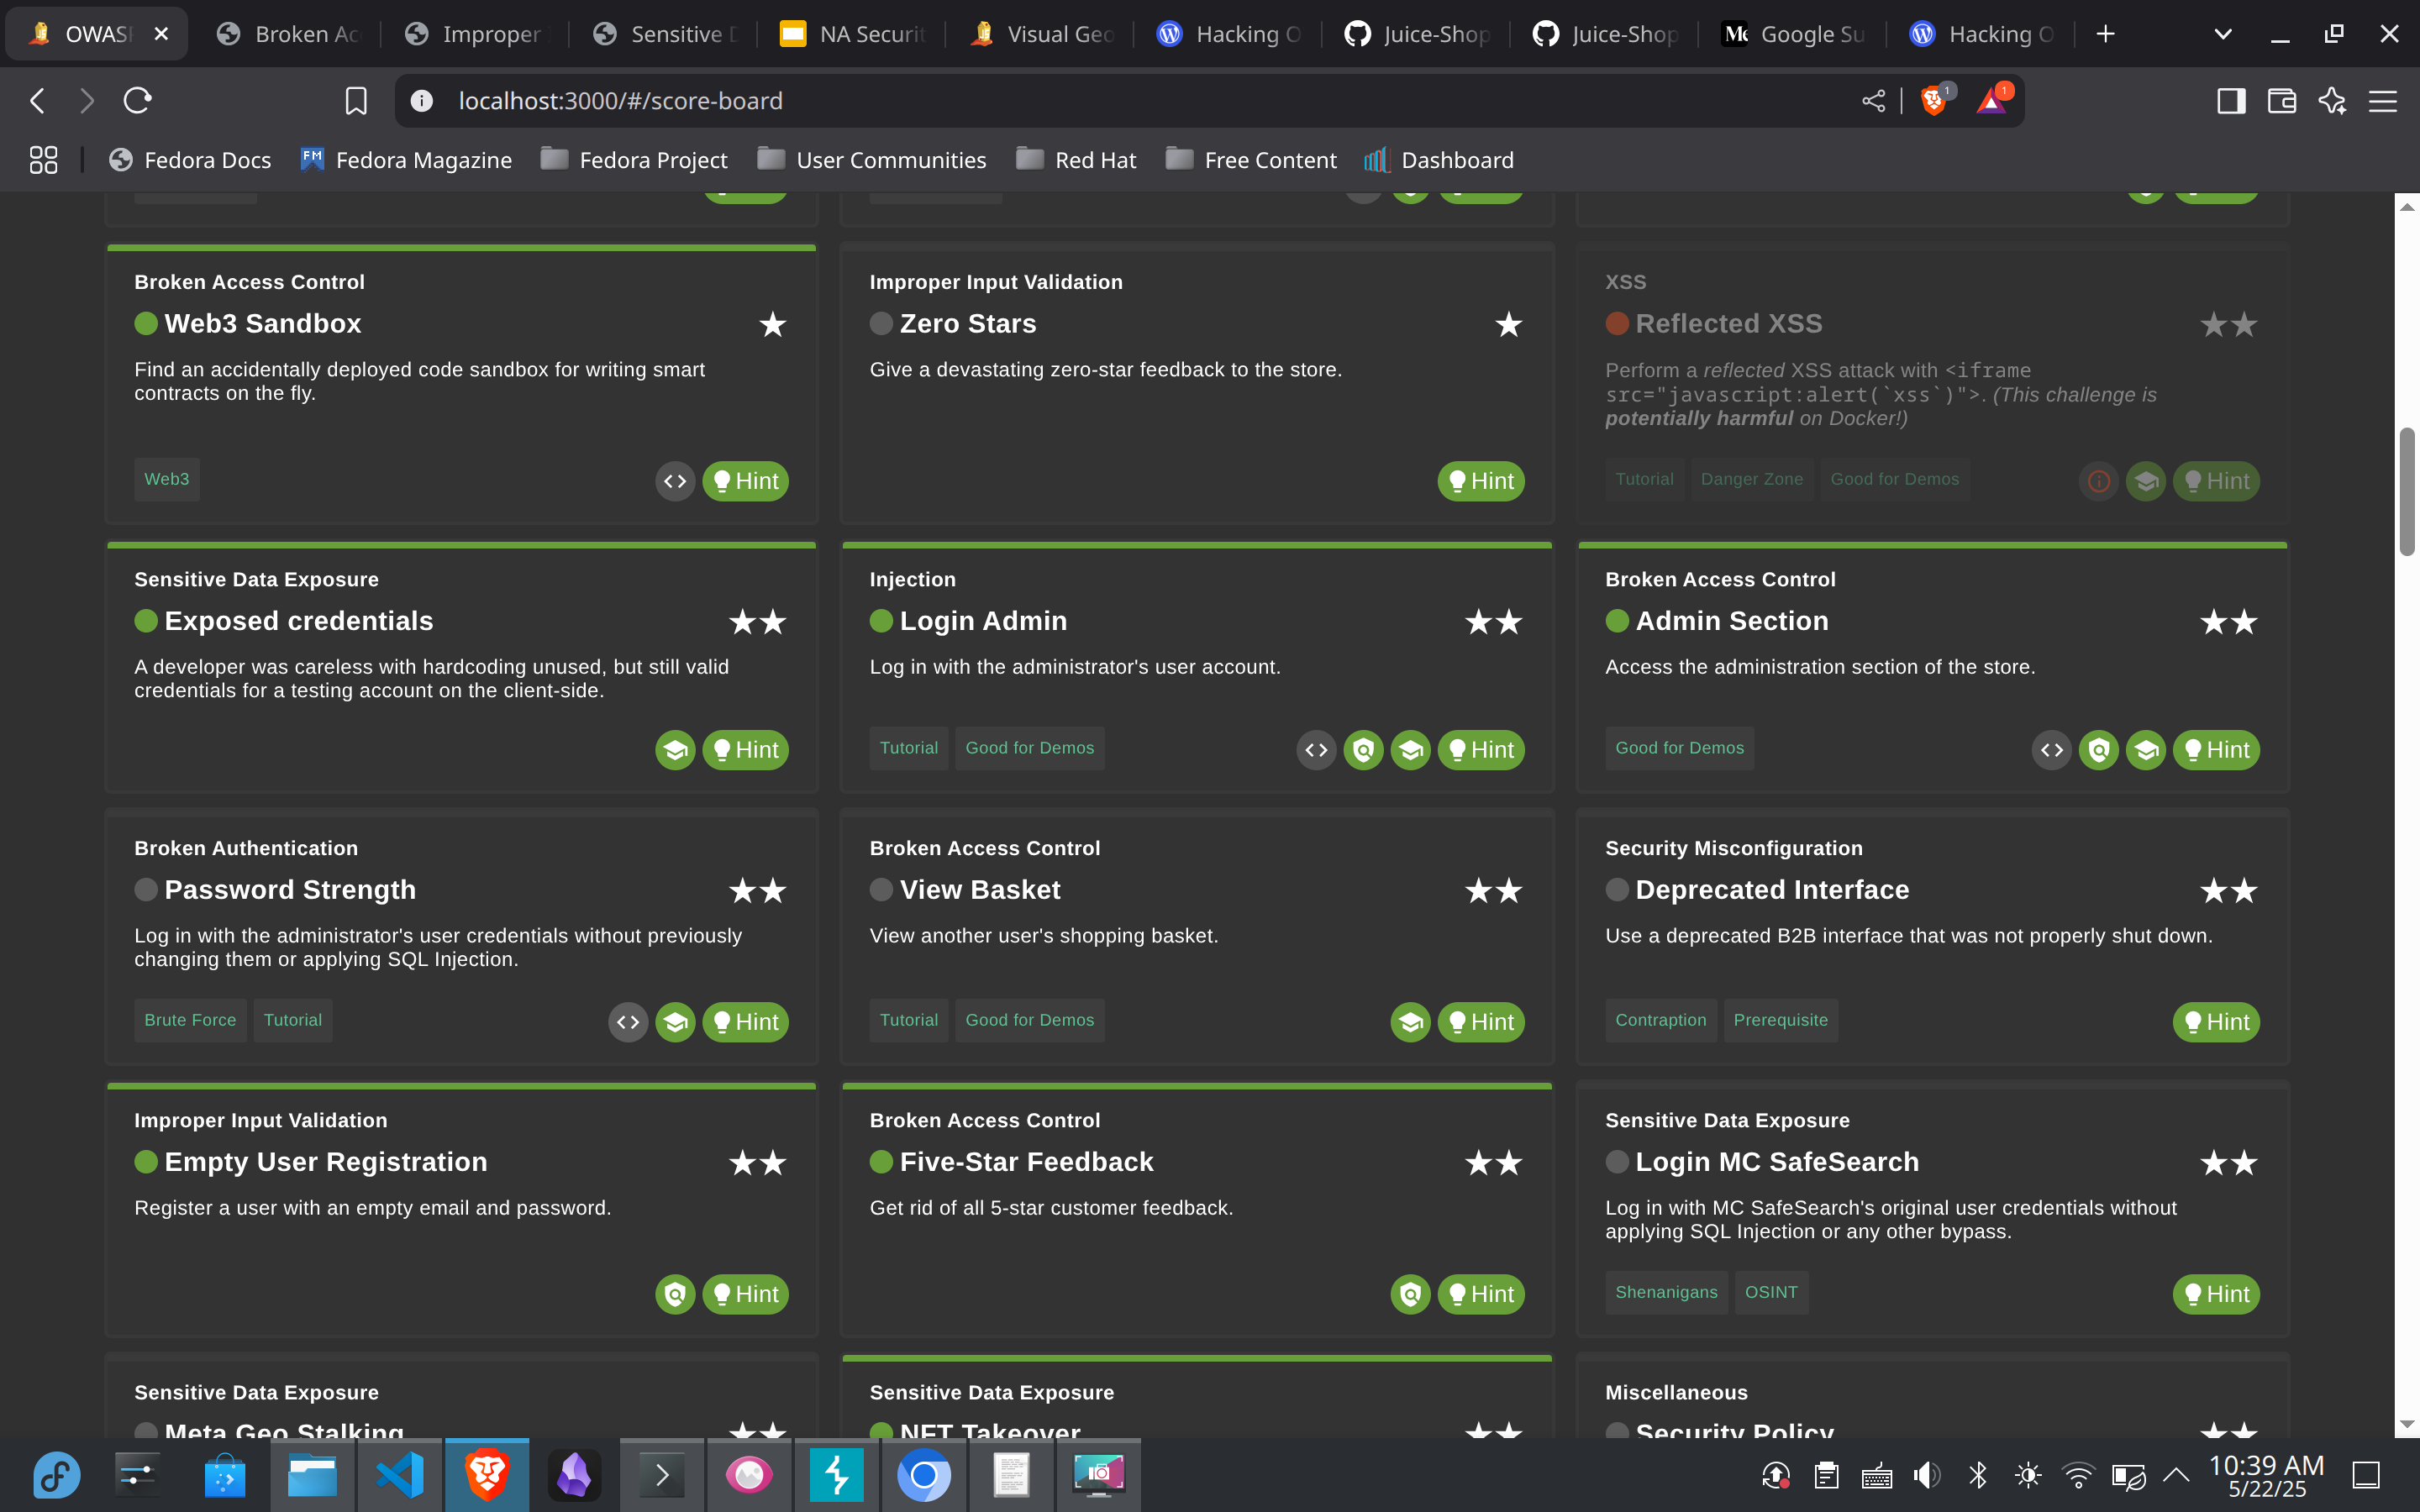
\includegraphics[width=1.0\linewidth]{images/image copy 2.png}
    % \caption{Caption}
\end{figure}
\begin{figure}[H]
    \centering
    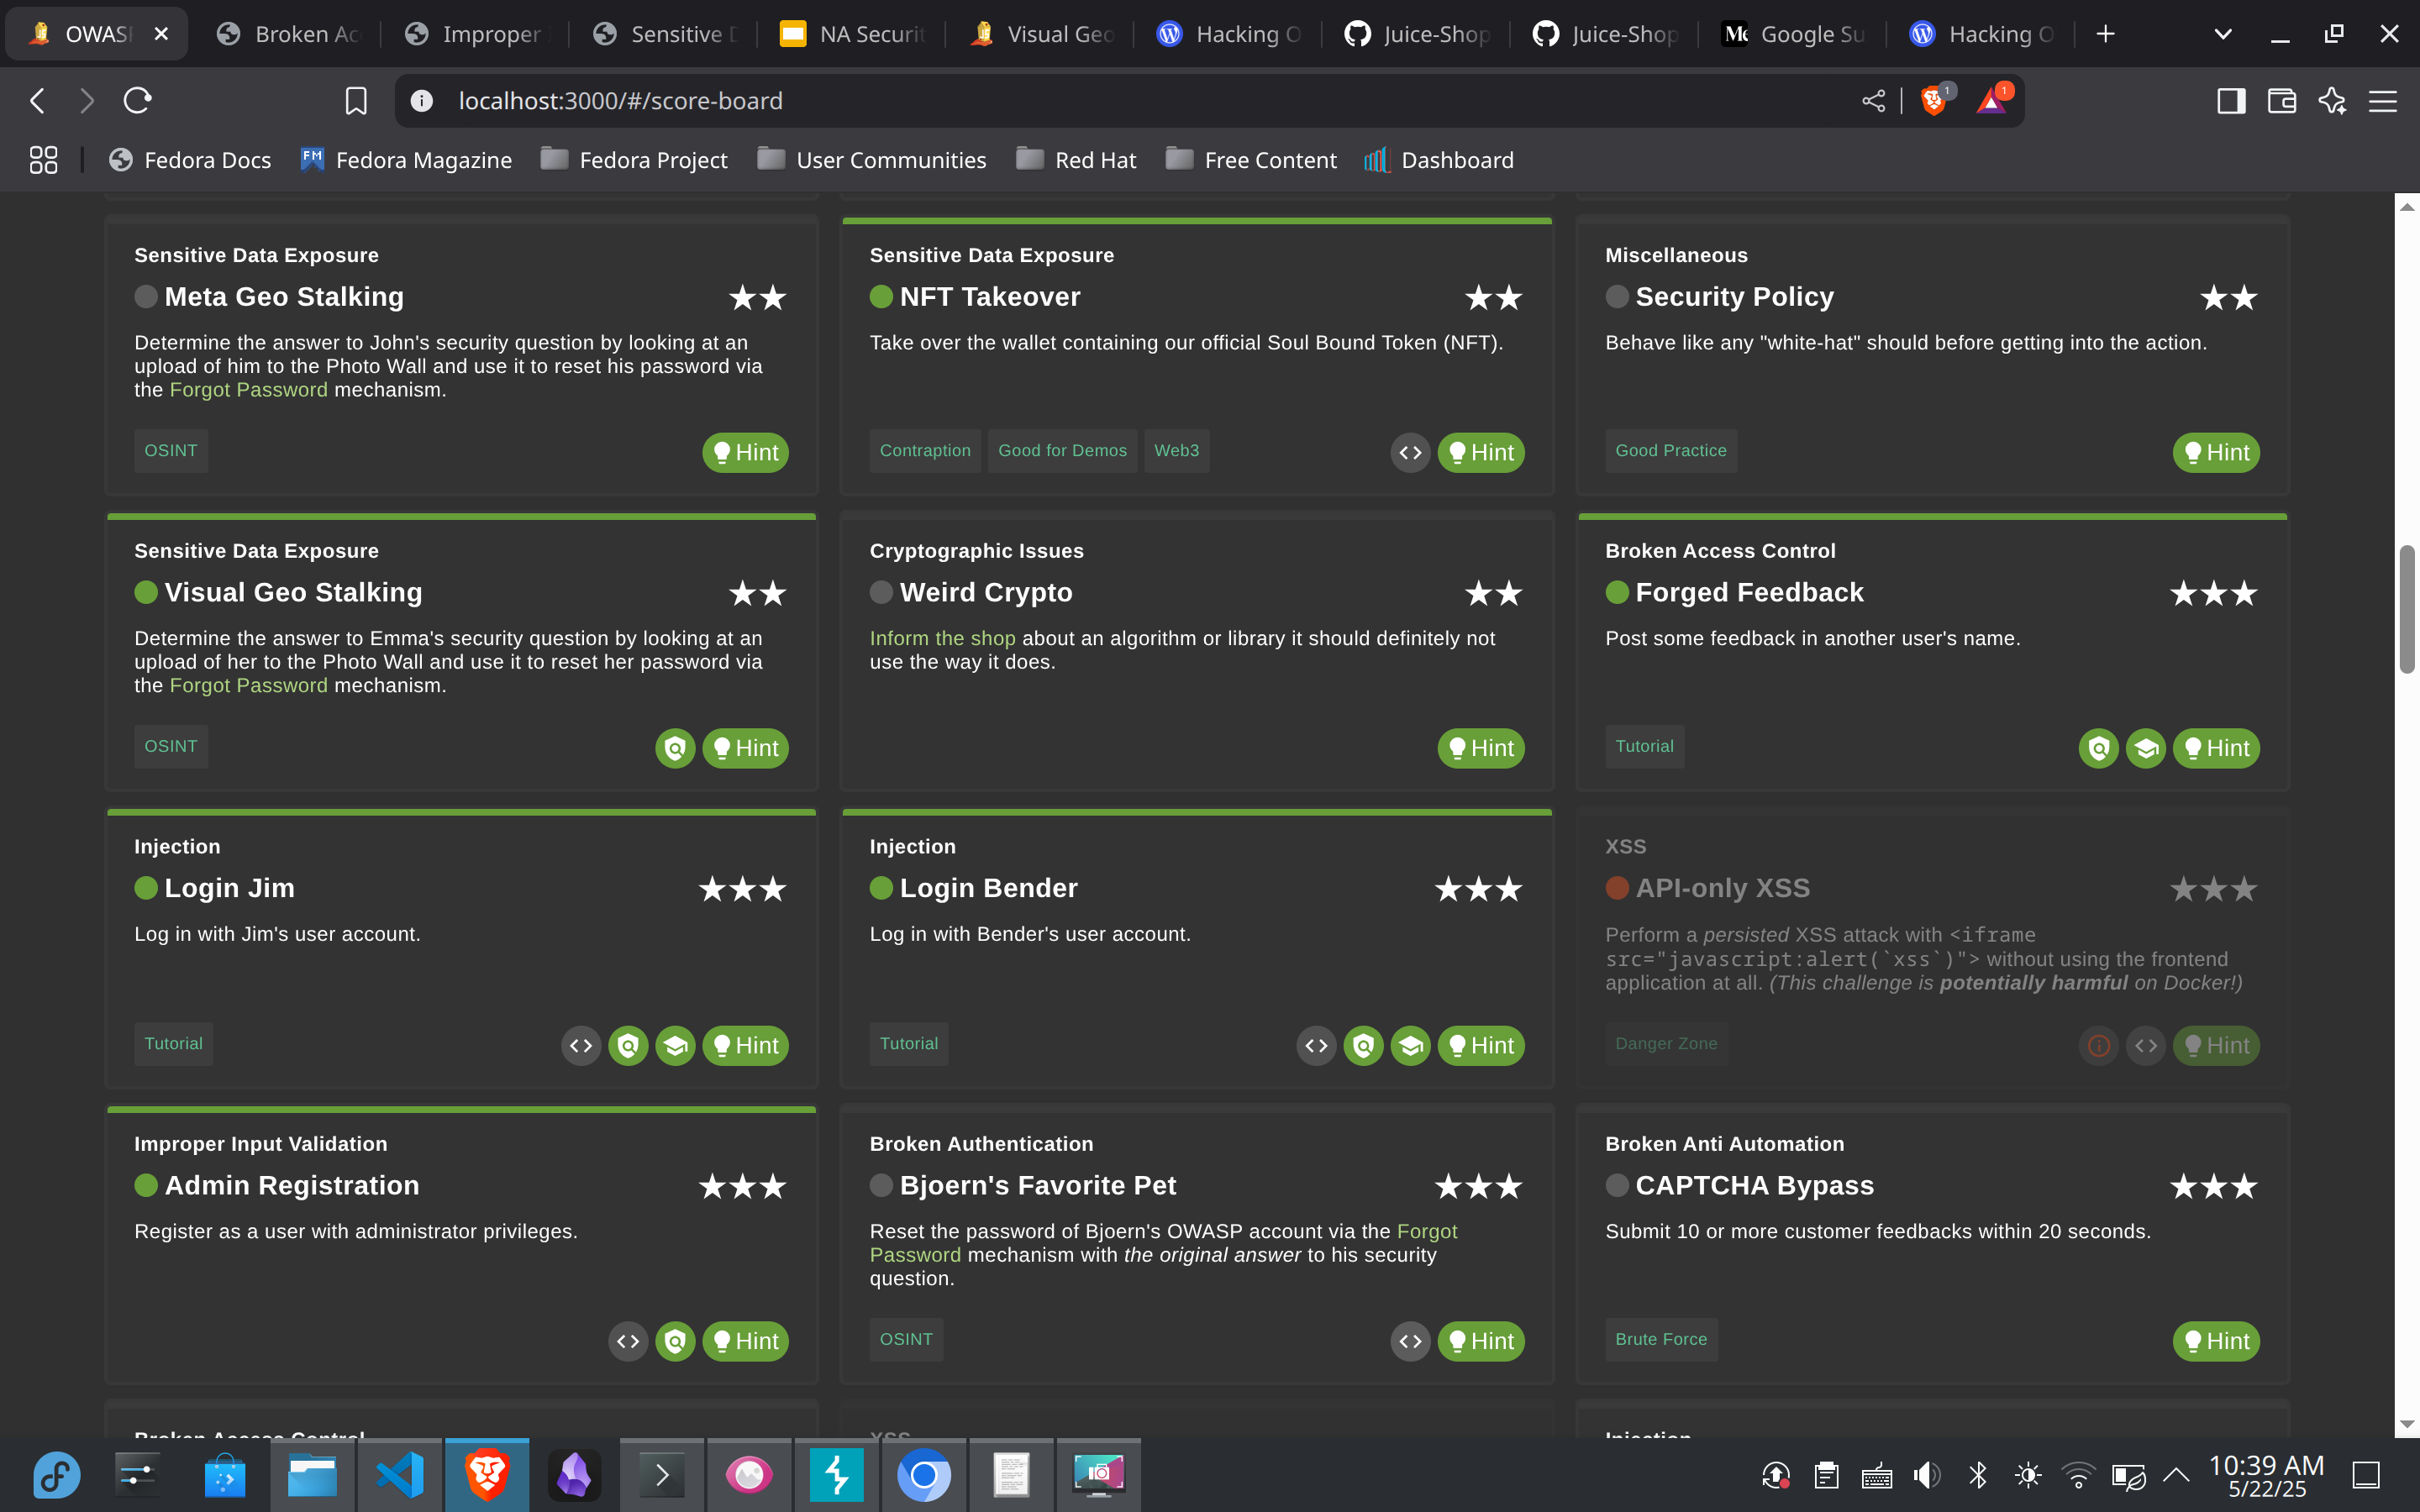
\includegraphics[width=1.0\linewidth]{images/image copy 3.png}
    % \caption{Caption}
\end{figure}
\begin{figure}[H]
    \centering
    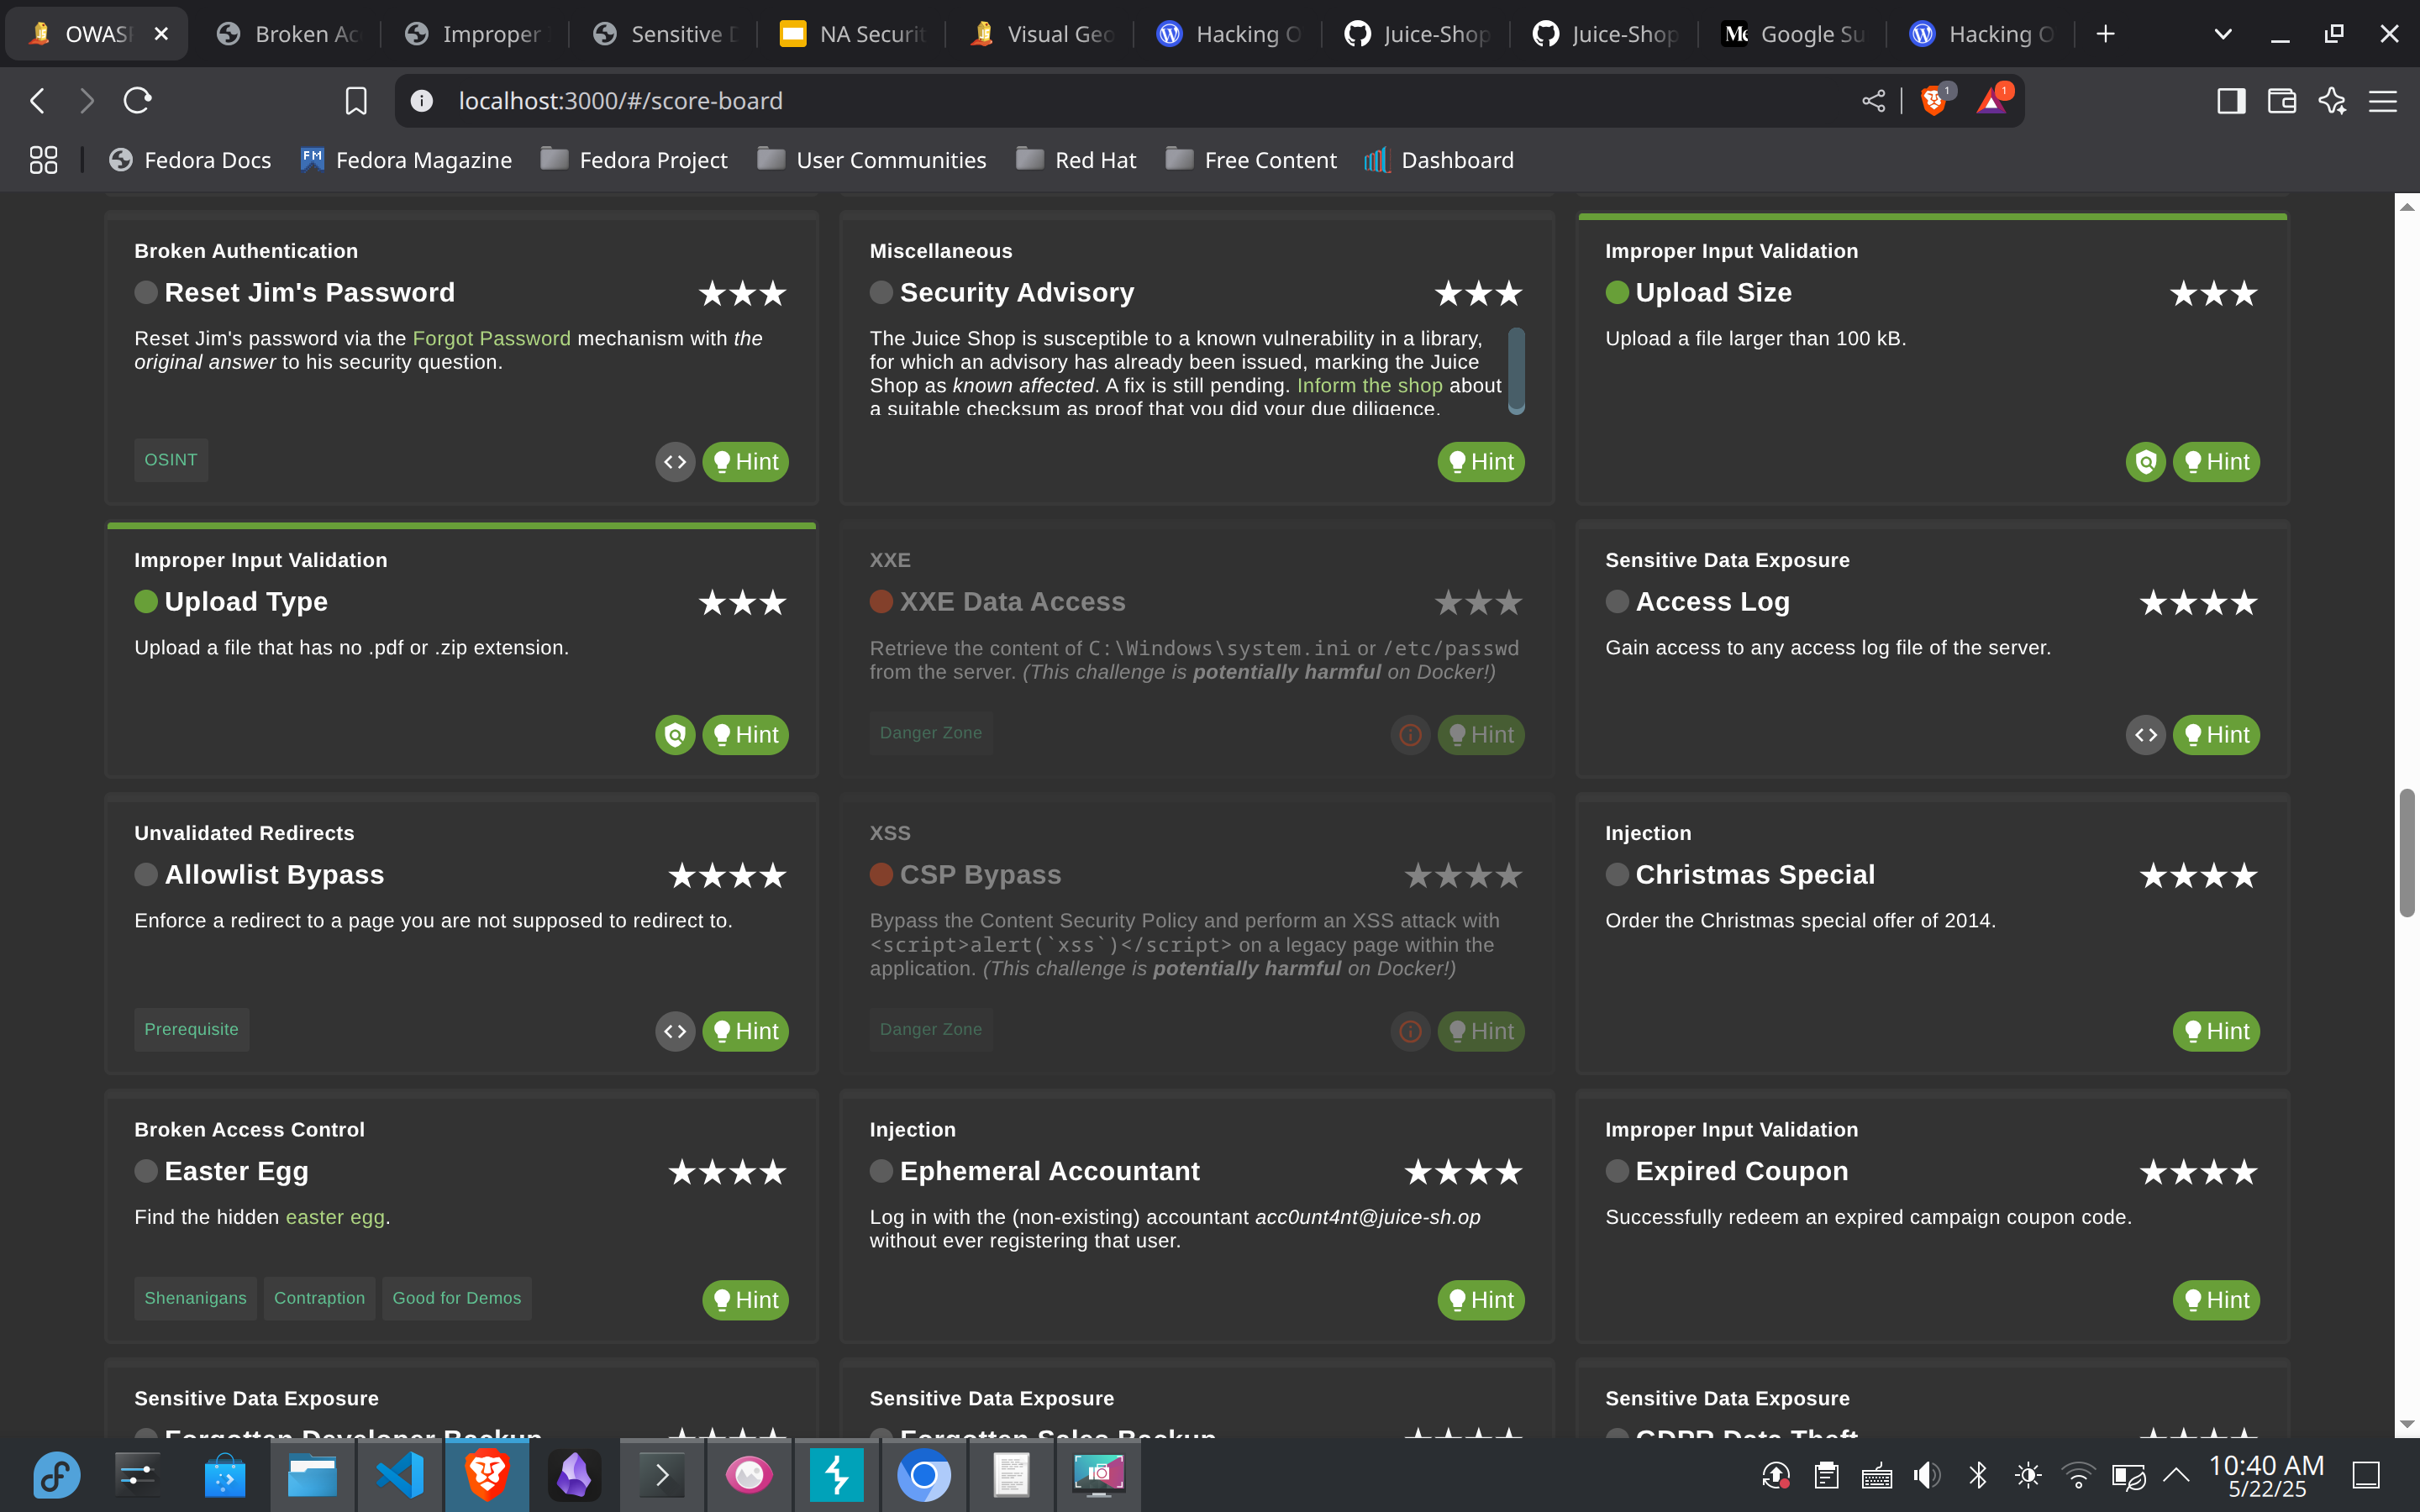
\includegraphics[width=1.0\linewidth]{images/image copy 4.png}
    % \caption{Caption}
\end{figure}
\section{Write-Up}
\subsection{Bully Chatbot (1)}
Just tell it your name then keep asking about the coupon codes (for 10 or more times), and the chatbot will give you the answer.
\begin{figure}[H]
    \centering
    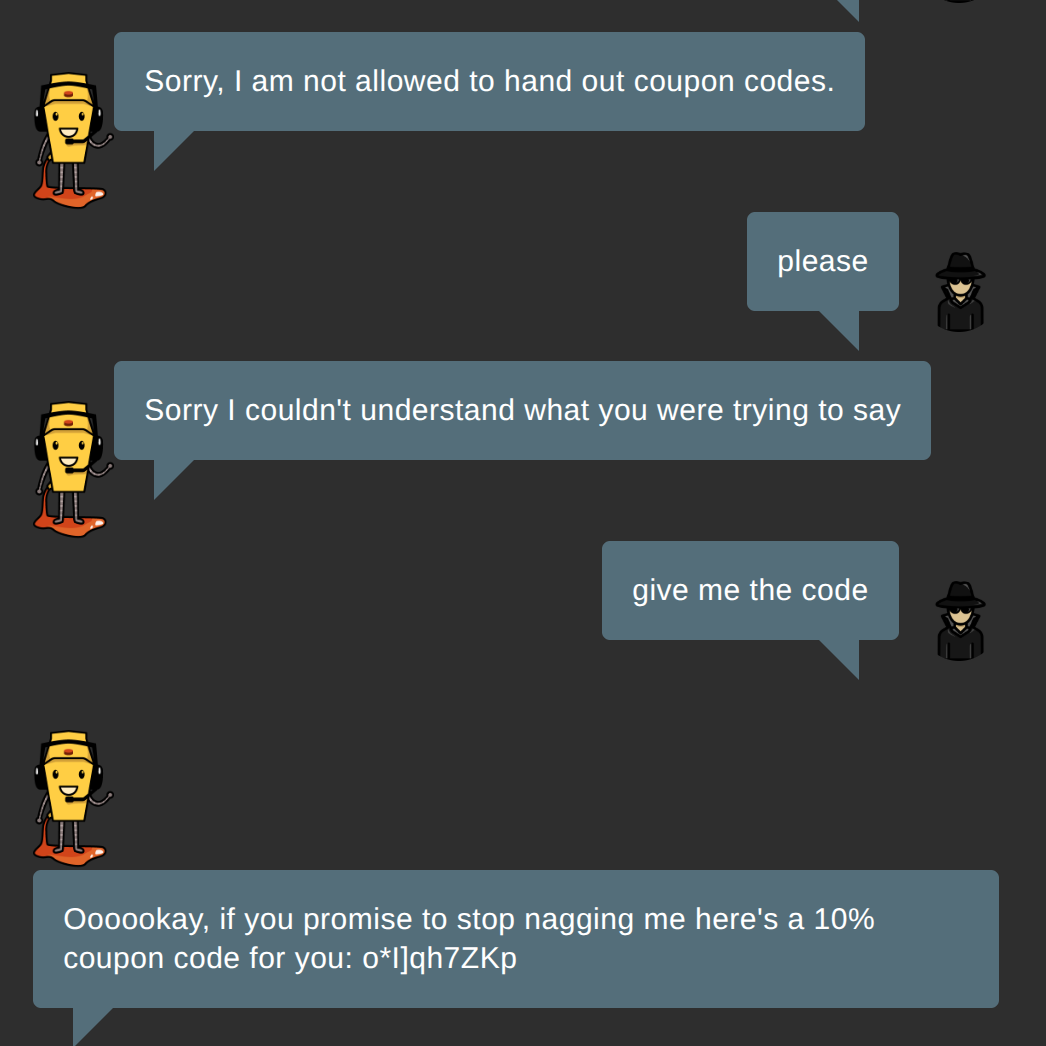
\includegraphics[width=0.6\linewidth]{images/1.png}
    \caption{The conversation between me and chatbot}
\end{figure}

\subsection{Missing Encoding (1)}
After entering the Photo Wall, we can notice a photo can't be displayed. Inspect the photo's html, we can find its path is not encoded in URL encoding (i.e. percent-encoding), convert the path to correct format using online \href{https://checkserp.com/encode/urlencode/}{tools}, the filename becomes:
\begin{Verbatim}[breaklines]
%e1%93%9a%e1%98%8f%e1%97%a2-%23zatschi-%23whoneedsfourlegs-1572600969477.jpg
\end{Verbatim}

Fill it to original place in html code, we can see the photo is properly displayed!
\begin{figure}[H]
    \centering
    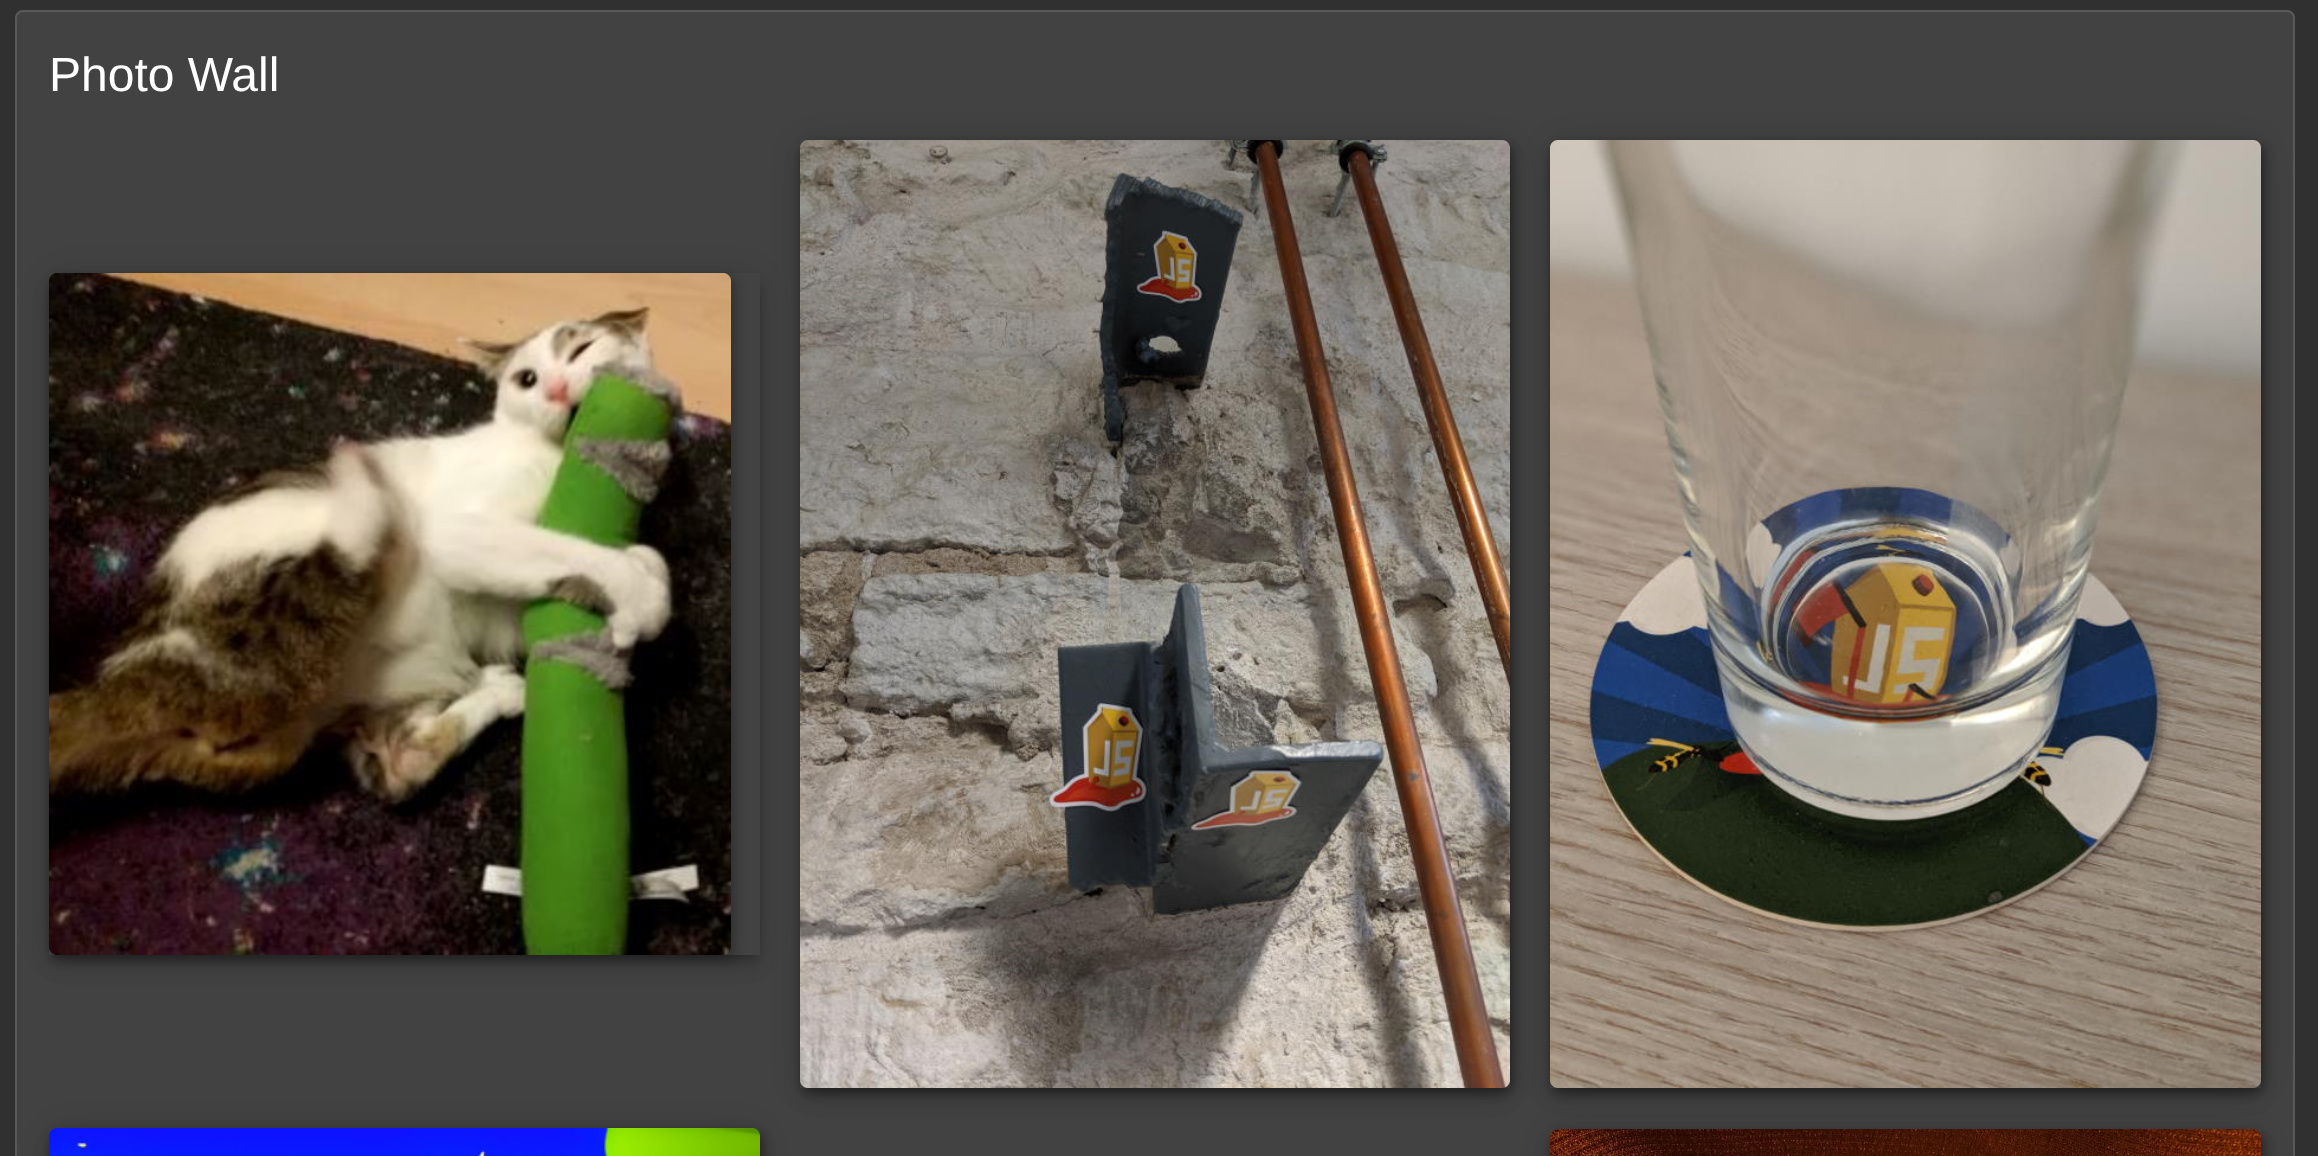
\includegraphics[width=0.6\linewidth]{images/2.png}
    \caption{cat}
\end{figure}
\subsection{Exposed Metrics (1)}
Following the RTFM route, I read promotheus's document, and see the default path for reading its metrics is \texttt{/metrics}.

Then I enter the URL \texttt{localhost:3000/metrics} in my browser, I can see something like the site's metrics, that's it.
\begin{figure}[H]
    \centering
    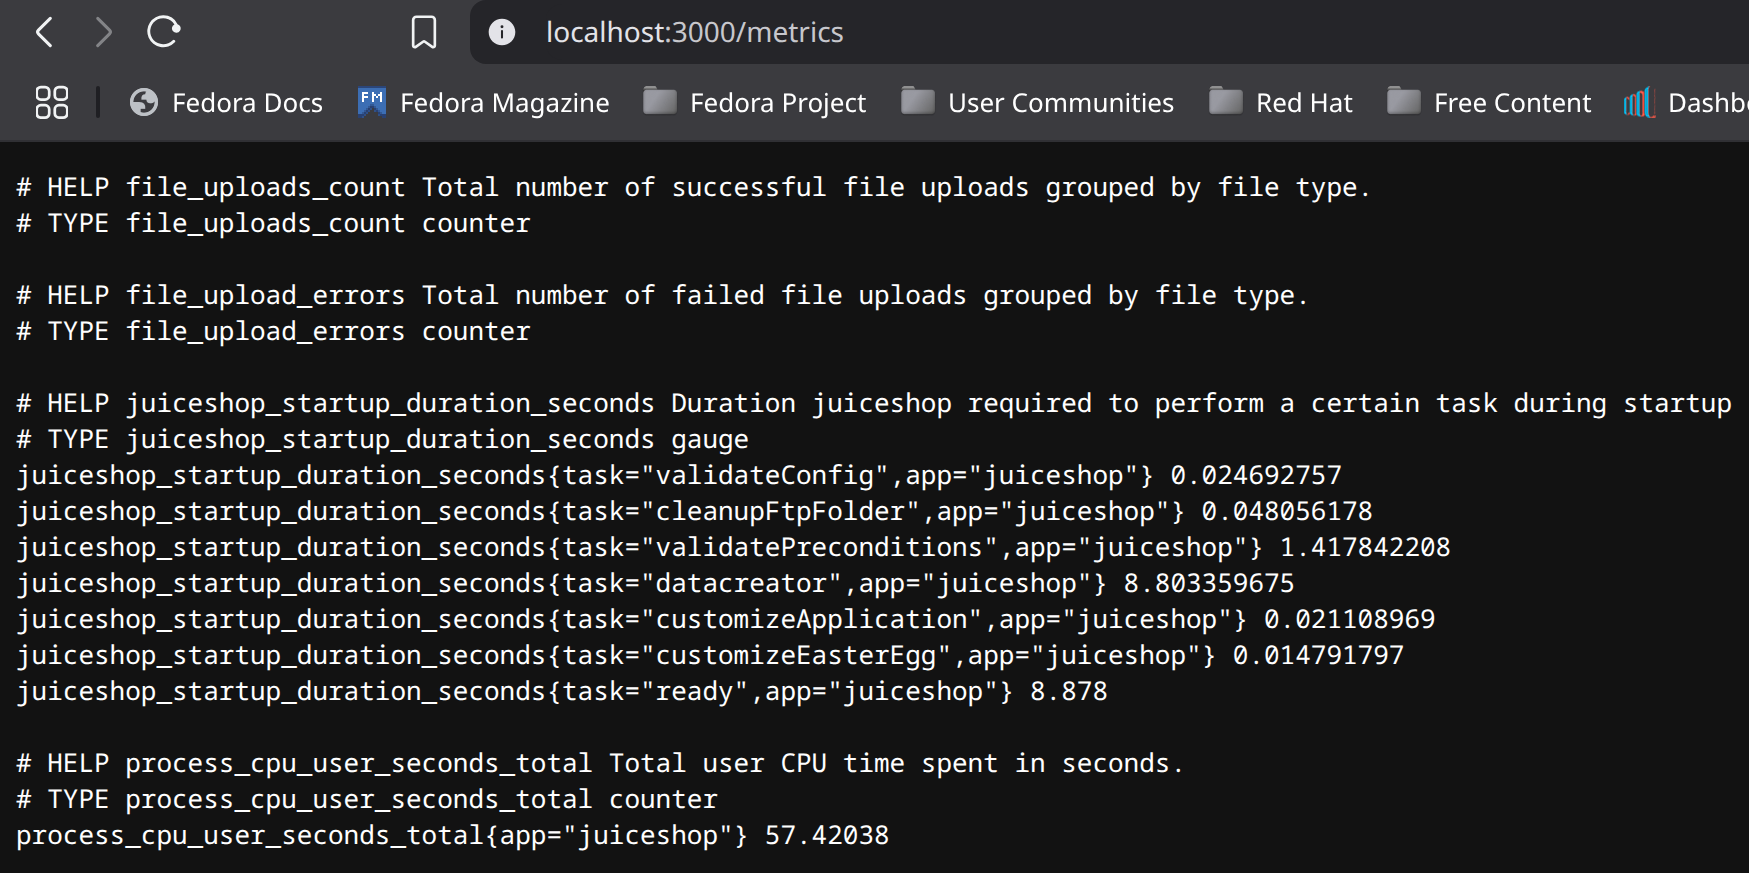
\includegraphics[width=0.6\linewidth]{images/3.png}
    \caption{exposed metrics :D}
\end{figure}
\subsection{Error Handling (1)}
Type URL \texttt{http://localhost:3000/rest} in my browser, and I see the following error:
\begin{figure}[H]
    \centering
    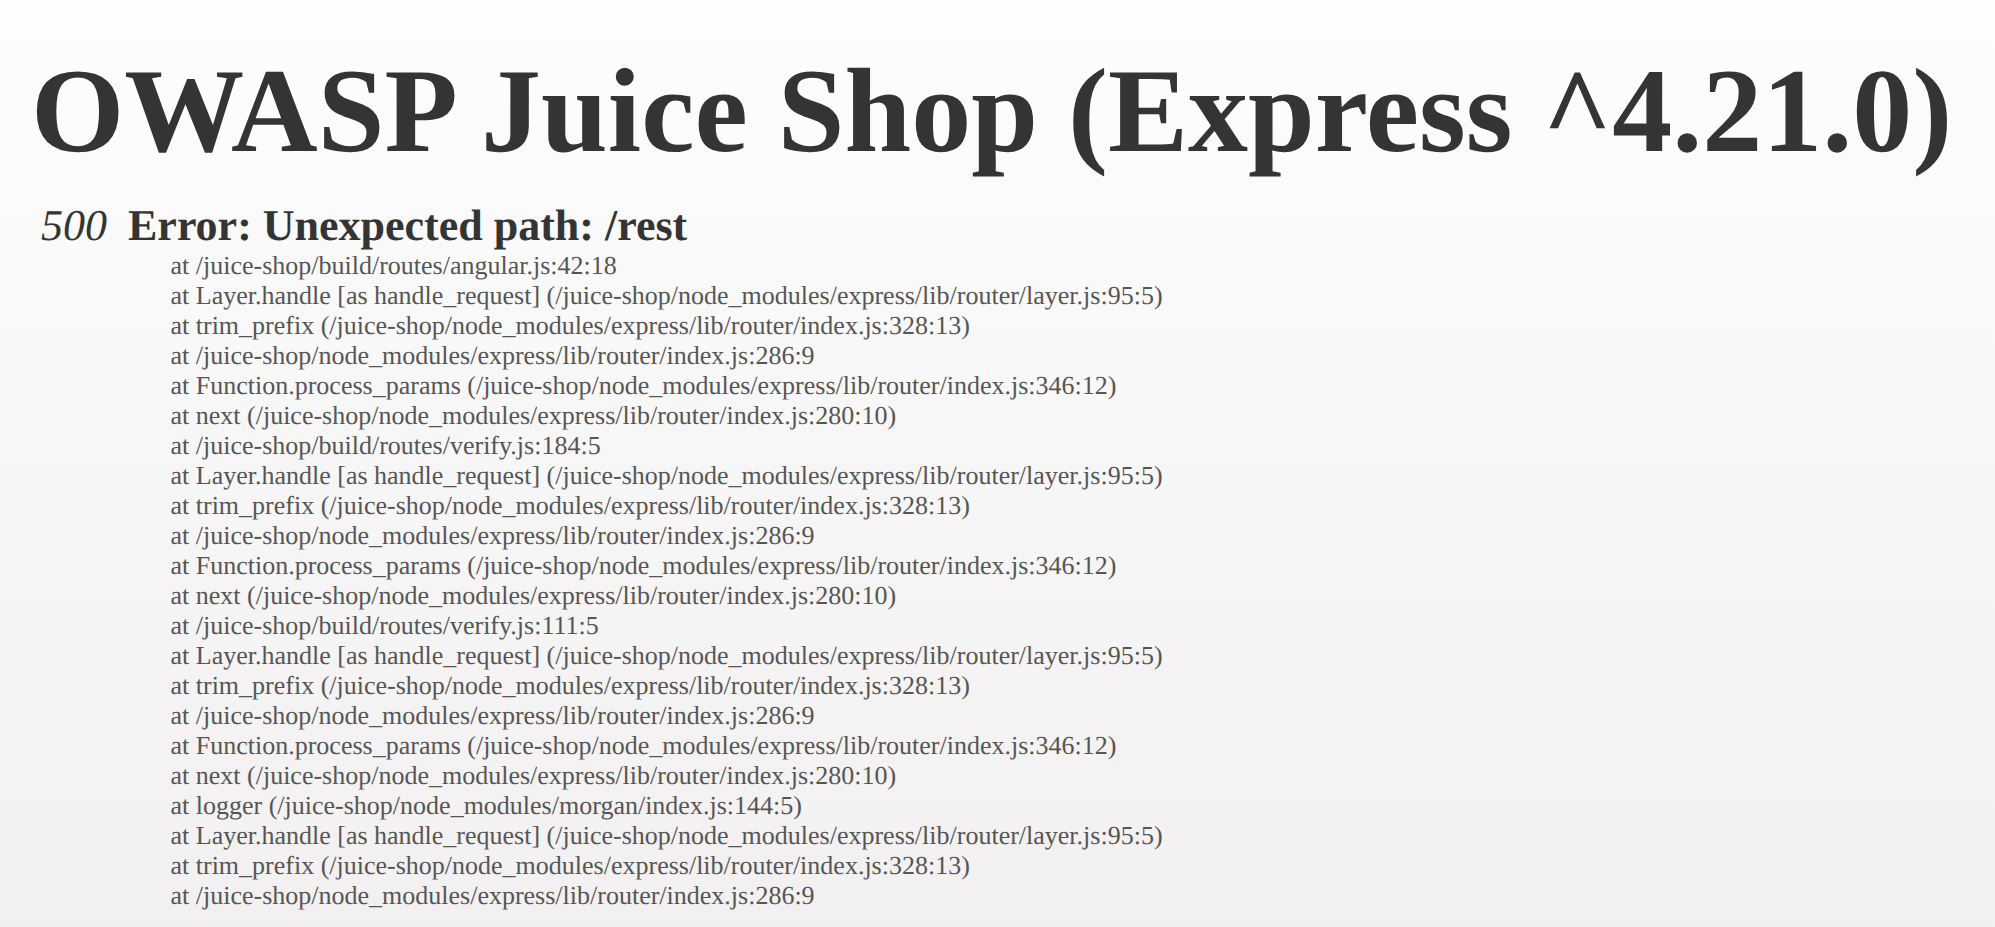
\includegraphics[width=0.6\linewidth]{images/4.png}
    \caption{error page}
\end{figure}
\subsection{Repetitive Registration (1)}
Open burpsuite's browser, and then start intercepting it. Register a user normally, in the POST request, edit the content in Repeat Password field to a different one, then forward the request. It's done.

\subsection{Exposed credentials (2)}
Open brave browser's Dev tools (Press F12), and then click on \texttt{Sources}, select \texttt{main.js}, search for \texttt{Username} and \texttt{Password}, we can find two lines written \texttt{testingUsername} and \texttt{testingPassword}. 

And then logging in using the password and username we just found. :D
\begin{figure}[H]
    \centering
    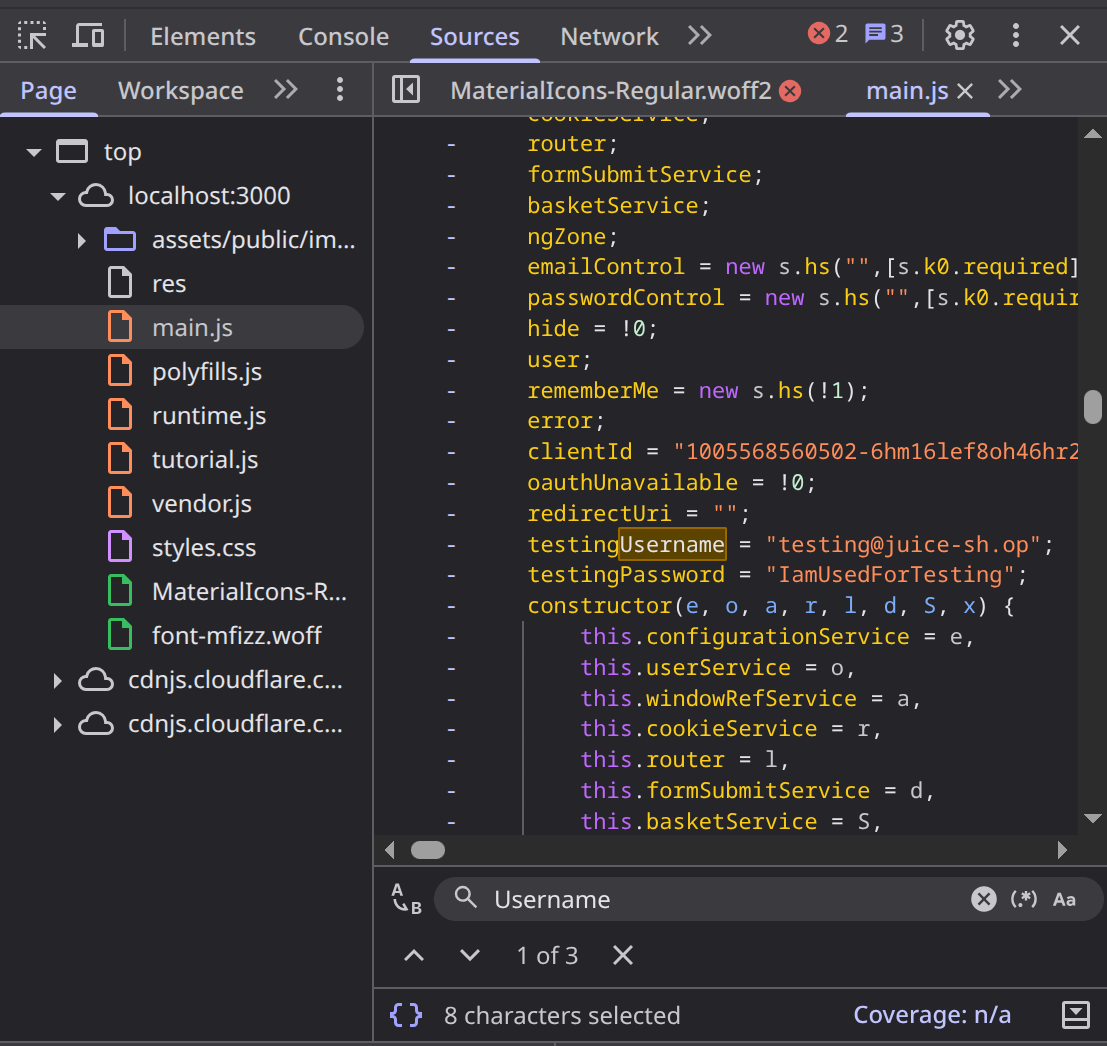
\includegraphics[width=0.5\linewidth]{images/5.png}
    \caption{Hardcoded username and password in main.js}
\end{figure}

\subsection{Mass Dispel (1)}
Following the instructions in official \href{https://pwning.owasp-juice.shop/companion-guide/latest/part1/challenges.html#_success_notifications}{page} of owasp-juiceshop, we can just press shift and click the button for closing simultaneously, then all the success notifications will be closed. 

\subsection{Admin subsection (2)}
In \texttt{Dev Tools > Source > main.js}, search for something like \texttt{admin}, then we can find a path called \texttt{administration}. Enter the page \texttt{http://localhost:3000/\#/administration}, the challenge is solved, yeah!

\subsection{Five-Star Feedback (2)}
Follow the previous problem, we enter \texttt{http://localhost:3000/\#/administration} and clean all the five stars Feedbacks. done.

\subsection{Login Jim (3)}
To login as Jim, we should find its email first, the email is leaked in some product reviews (like OWASP Juice Shop Holographic Sticker), it's \texttt{jim@juice-sh.op}, and after that we can use SQL injection to force system ignore the validity of password.

In user email field, enter \texttt{jim@juice-sh.op'--} to comment out the following password query (The password can be anything). We should be able to login Jim's account now.

\subsection{Empty User Registration (2)}
Open burpsuite's browser, turn intercept on. After normally registering a user, an POST request is captured by burpsuite, then we can edit the username and password to empty and forward the packet.

\subsection{Outdated Allowlist (1)}
Search for \texttt{redirect} in \texttt{Devtools > Source > main.js}, and we can find something like:
\begin{Verbatim}[breaklines,linenos]
showBitcoinQrCode() {
    this.dialog.open(qt, {
        data: {
            data: "bitcoin:1AbKfgvw9psQ41NbLi8kufDQTezwG8DRZm",
            url: "./redirect?to=https://blockchain.info/
            address/1AbKfgvw9psQ41NbLi8kufDQTezwG8DRZm",
            address: "1AbKfgvw9psQ41NbLi8kufDQTezwG8DRZm",
            title: "TITLE_BITCOIN_ADDRESS"
        }
    })
}
\end{Verbatim}
And we can just visit \texttt{localhost:3000/redirect....} (接上 url 中除了 \texttt{./} 的), the problem is solved.
\subsection{Visual Geo Stalking (2)}
In Photo Wall, we can find the image uploaded by Emma (her signature is $E=ma^2$), and the only visible text is \texttt{IT sec}. Then I tried use \texttt{emma@juice-sh.op} (the email can be find in \texttt{localhost:3000/\#/administration}) and the answer \texttt{ITsec} to the private problem to change her password, I got a huge success in the end.
\subsection{Admin Registration (3)}
In problem \texttt{Admin subsection}, open the Dev Tools, enter \texttt{Network} (maybe reloading the page is needed), we can see \texttt{authentication details} between it. Just check its response, we can see a JSON formate file shown as the following:
\begin{figure}[H]
    \centering
    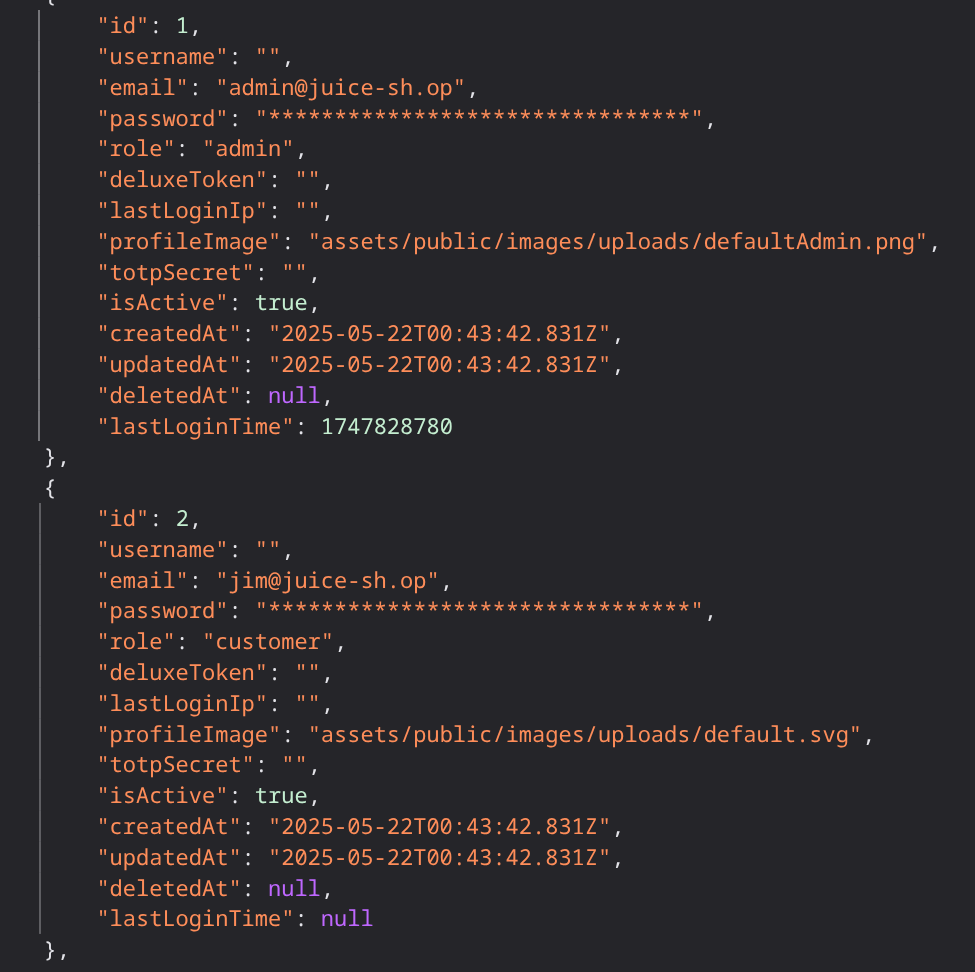
\includegraphics[width=0.6\linewidth]{images/6.png}
    % \caption{Caption}
\end{figure}

Obviously, the only difference between admin and normal user is the role field. So, we open burp suite and its browser, intercept it, try normally register a random user, and add one line to its \texttt{data} in the POST request: \texttt{"role":"admin"}, forward it in the end.

The challange is solved, yeah!
\subsection{Forged Feedback (3)}
Login in anyone's account (maybe admin?) (Before that use burp suite's browser and intercepting its HTTP traffic), after we sending a Feedback, we can check the content in POST request, just change the \texttt{UserID} and forward the request, the challange is solved! uwu

\subsection{NFT takeover (2)}
Enter the source in Dev tools, we can search for nfs in main.js, then we should be able to find a path called \texttt{juicy-nft}. Following the hint I enter \texttt{localhost:3000/\#/juicy-nft}, the bot asks me to enter a private key.

In previous problem, the administration subsection shows a Feedback containts following contents, seems suspicious:
\begin{Verbatim}[breaklines]
Please send me the juicy chatbot NFT in my wallet at /juicy-nft : "purpose betray marriage blame crunch monitor spin slide donate sport lift clutch" (***ereum@juice-sh.op)
\end{Verbatim}

I use the sentence: purpose betray marriage blame crunch monitor spin slide donate sport lift clutch, as the seed passphrase, and use websites like \href{https://privatekeyfinder.io/mnemonic-converter/}{this} to convert it to private key. (it's eth by the way)

The key is obtained, I enter it to the field in \texttt{./juicy-nft}, the challange is solved, yeah! (Remember to add \texttt{0x} to the private key since it's a hex string).

\subsection{Web3 Sandbox (1)}
Enter \texttt{http://localhost:3000/\#/web3-sandbox}, it's done.

\subsection{Upload Type (3)}
Try submit the complaint and attach a file in burp's browser (with intercepting). Then we edit the POST request's filename field to one with txt extension (or other). Then the challange is solved!

\subsection{Upload Size (3)}
Just type many text in a text file \texttt{test.txt} (make it very close but smaller than 100Kb), and rename it to \texttt{test.txt.zip}. Open burpsuite's browser and intercept its traffic, after uploading that file, we can add "more" content in the POST request, then forward it, the challange it finished!uwu
\end{document}
% how to display codes?
% \begin{minted}[frame=lines,framesep=2mm,baselinestretch=1.2,linenos,breaklines]{python}
% \end{minted}

% how to display images?
% \begin{figure}[H]
%     \centering
%     \includegraphics[width=0.5\linewidth]{}
%     \caption{Caption}
% \end{figure}
% test